% 1977 q9 solution: rectangle with auxiliary dashed extension
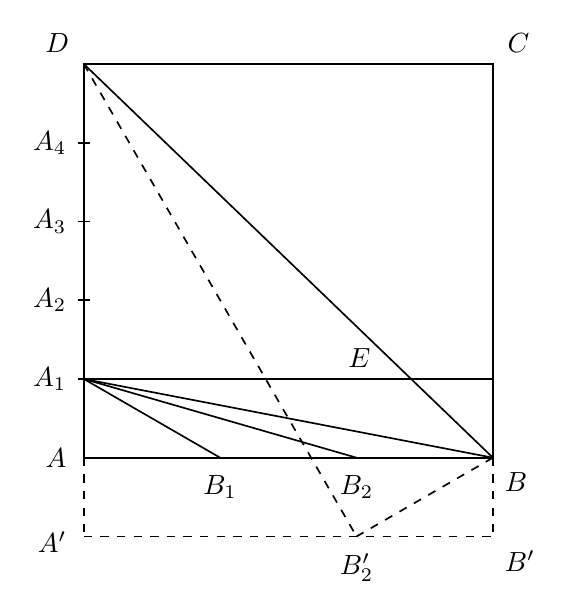
\begin{tikzpicture}[x=1cm,y=1cm,font=\normalsize,line width=.6pt,
  geom/.style={solid,line width=.6pt},
  hid/.style={dashed,line width=.6pt},
  lbl/.style={font=\normalsize,inner sep=2pt}]
% main rectangle A(0,0) B(5.1961524227,0) C(5.1961524227,5) D(0,5), a=1 unit
\coordinate (A) at (0,0);
\coordinate (B1) at (1.7320508076,0);
\coordinate (B2) at (3.4641016151,0);
\coordinate (B) at (5.1961524227,0);
\coordinate (C) at (5.1961524227,5);
\coordinate (D) at (0,5);
\coordinate (A1) at (0,1);
\coordinate (A2) at (0,2);
\coordinate (A3) at (0,3);
\coordinate (A4) at (0,4);
\foreach \k in {1,2,3,4} {\draw (-.08,\k)--(.08,\k);}
% extension dashed
\coordinate (Apr) at (0,-1);
\coordinate (B2pr) at (3.4641016151,-1);
\coordinate (Bpr) at (5.1961524227,-1);
\draw[geom] (A)--(B)--(C)--(D)--cycle;
\draw[geom] (A1)--(B);
\draw[geom] (A1)--(B1);
\draw[geom] (A1)--(B2);
\draw[geom] (D)--(B);
\draw[hid] (D)--(B2pr);
\draw[hid] (B)--(B2pr);
\draw[hid] (A)--(Apr);
\draw[hid] (Apr)--(Bpr);
\draw[hid] (B)--(Bpr);
% horizontal A1-E line (E intersection with DB implicit)
\draw[geom] (A1)--(5.1961524227,1);
\node[lbl,left,xshift=-4pt] at (A) {$A$};
\node[lbl,left,xshift=-4pt] at (A1) {$A_1$};
\node[lbl,left,xshift=-4pt] at (A2) {$A_2$};
\node[lbl,left,xshift=-4pt] at (A3) {$A_3$};
\node[lbl,left,xshift=-4pt] at (A4) {$A_4$};
\node[lbl,above left,xshift=-3pt,yshift=2pt] at (D) {$D$};
\node[lbl,above right,xshift=3pt,yshift=2pt] at (C) {$C$};
\node[lbl,below,yshift=-4pt] at (B1) {$B_1$};
\node[lbl,below,yshift=-4pt] at (B2) {$B_2$};
\node[lbl,below right,xshift=2pt,yshift=-3pt] at (B) {$B$};
\node[lbl,left,xshift=-4pt,yshift=-2pt] at (Apr) {$A'$};
\node[lbl,below,yshift=-4pt] at (B2pr) {$B'_2$};
\node[lbl,below right,xshift=2pt,yshift=-3pt] at (Bpr) {$B'$};
\node[lbl,above,yshift=2pt] at (3.5,1) {$E$};
\end{tikzpicture}

